\documentclass[oneside]{estilo}

% ---------------------------------------------------------------------------
% PACOTES
% ---------------------------------------------------------------------------
\usepackage[alf, abnt-emphasize=bf, recuo=0cm, abnt-etal-cite=2, abnt-etal-list=0]{abntex2cite}  % Citações ABNT
\usepackage[utf8]{inputenc}                         % Acentuação direta
\usepackage[T1]{fontenc}                            % Codificação da fonte em 8 bits
\usepackage{graphicx}                               % Inserir figuras
\usepackage{amsfonts, amssymb, amsmath}             % Fonte e símbolos matemáticos
\usepackage{booktabs}                               % Comandos para tabelas
\usepackage{verbatim}                               % Texto literal
\usepackage{multirow, array}                        % Múltiplas linhas e colunas em tabelas
\usepackage{indentfirst}                            % Endenta o primeiro parágrafo de cada seção
\usepackage{microtype}                              % Melhorias de justificação
\usepackage[algoruled, portuguese]{algorithm2e}     % Algoritmos
\usepackage{float}                                  % Floats
%\usepackage{times}                                 % Usa a fonte Times

\usepackage{color}
\usepackage{chronosys}
\usepackage{pdflscape}
%\usepackage{tabu}                                  % deixado comentado (evita erro se não instalado)
\usepackage{makecell}
\usepackage{nameref}
\usepackage{listings}
\usepackage{enumitem}
\usepackage{chngcntr}
\usepackage{colortbl}
\usepackage[htt]{hyphenat}
\usepackage{mdframed}

\mdfsetup{skipabove=1.5\topskip,skipbelow=0.5\topskip}
\mdfdefinestyle{pp}{%
	linecolor=black,
	outerlinewidth=.5pt,
	roundcorner=5pt,
	innertopmargin=8pt,
	innerbottommargin=0.5\baselineskip,
	usetwoside=false
}

%\usepackage{minitoc}
%\dominitoc% Initialization

\newcommand{\enumerateletter}[2]{\textbf{#1\textsubscript{#2}}}

% ---------------------------------------------------------------------------
% PREÂMBULO DO DOCUMENTO  (usa \input, NÃO \include)
% ---------------------------------------------------------------------------
%
% Documento: Preâmbulo + Capa
%

% -------------------------------
% Pacotes necessários
% -------------------------------
\usepackage{lmodern}
\usepackage{listings}
\usepackage{tocloft}
\usepackage{chngcntr}
\usepackage{tabularx}
\usepackage{booktabs}
\usepackage{array}

% -------------------------------
% Configuração de listagens
% -------------------------------
\renewcommand{\lstlistingname}{Código}

% Numeração contínua já configurada no estilo.cls
% (não duplicar aqui)

% Criação da "Lista de Códigos" conforme ABNT
\begingroup\makeatletter
\let\newcounter\@gobble
\let\setcounter\@gobbletwo
\globaldefs\@ne
\let\c@loldepth\@ne
\newlistof{listings}{lol}{\lstlistlistingname}
\newlistentry{lstlisting}{lol}{0}
\endgroup

\renewcommand{\cftlstlistingaftersnum}{\hfill--\hfill}

\let\oldlstlistoflistings\lstlistoflistings
\renewcommand{\lstlistoflistings}{%
  \begingroup%
  \let\oldnumberline\numberline%
  \renewcommand{\numberline}{\lstlistingname\space\oldnumberline}%
  \oldlstlistoflistings%
  \endgroup}

% Estilo para códigos
\lstdefinestyle{master-thesis}{
  basicstyle=\ttfamily\small,
  numbers=left,
  numberstyle=\tiny,
  frame=tb,
  columns=fullflexible,
  showstringspaces=false,
  captionpos=b,
  breaklines=true,
  tabsize=2
}
\lstset{style=master-thesis}

% -------------------------------
% ==== DADOS DA CAPA ====
% -------------------------------

\instituicao{CENTRO UNIVERSITÁRIO DE OURINHOS}
\departamento{CURSO: ENGENHARIA DE SOFTWARE}
\titulotb{Plataforma Web para Gestão de Escritórios de Advocacia}

\nomeautor{%
  \textbf{Gabriel De Oliveira Cordeiro}\\
  \textbf{José Gabriel Celso Lima}\\
  \textbf{Laís de Oliveira}\\
  \textbf{Milena Maria Romano da Silva}%
}

\localapresentacao{Ourinhos -- São Paulo}
\anoapresentacao{2026}

\usepackage[a4paper, top=3.0cm, bottom=2.0cm, left=3.0cm, right=2.0cm]{geometry}

\newcommand{\blue}[1]{\textcolor{blue}{#1}}       % proposed
\newcommand{\red}[1]{\textcolor{red}{#1}}         % to be removed
\newcommand{\green}[1]{\textcolor{green}{#1}}     % to be discussed?
\newcommand{\magenta}[1]{\textcolor{magenta}{#1}} % warning

\settocdepth{subsection}

% ---------------------------------------------------------------------------
% HIPERLINKS / PDF
% ---------------------------------------------------------------------------
\makeatletter
\hypersetup{
    portuguese,
    colorlinks,
    linkcolor=blue,
    citecolor=blue,
    filecolor=black,
    urlcolor=black,
    breaklinks=true,
    pdftitle={\imprimirtitulotb},
    pdfauthor={\imprimirnomeautor}
}
\makeatother

\renewcommand{\algorithmautorefname}{Algoritmo}
\def\equationautorefname~#1\null{Equa\c c\~ao~(#1)\null}

\makeindex


\begin{document}
 
    \frenchspacing

    \pretextual
    \include{01-elementos-pre-textuais/dados}
    %
% Documento: Capa
%

\makeatletter
\begin{capa}
	\thispagestyle{empty}%limpa estilo da pagina
	\setlength{\baselineskip}{0.72\baselineskip}
    \begin{center} %Alinhamento centralizado
	

    \textbf{\expandafter\uppercase\expandafter{\imprimirinstituicao}}\\
    \textbf{\expandafter\uppercase\expandafter{\imprimirdepartamento}}\\
    %\textbf{\expandafter\uppercase\expandafter{\imprimirprograma}}\\
	\vspace*{5cm}%Espaçamento entre linhas
	\large\textbf{\expandafter\uppercase\expandafter{\imprimirtitulotb}}\\
	\vspace*{6cm}%Espaçamento entre linhas	
	\small\textbf{\expandafter\uppercase\expandafter{\imprimirnomeautor}}\\
	\vspace*{6.5cm}%%Espaçamento entre linhas
	\large\textbf{\expandafter\expandafter{\imprimirlocalapresentacao, \imprimirdataapresentacao}}
	%\small\textbf{\expandafter\uppercase\expandafter{\imprimirdata}}\\
		
		
		
	\end{center} %Alinhamento centralizado
\end{capa}
\makeatother

	


    \include{01-elementos-pre-textuais/resumoPt}
    %
% Documento: Resumo (Inglês)
\begin{RESUMO}
\thispagestyle{empty}
A rotina de um escritório de advocacia envolve o acompanhamento de processos, o controle de prazos, a organização de documentos e o cadastro de clientes. Quando essas atividades são realizadas de forma manual, 
podem ocorrer perda de prazos, dificuldade no acesso às informações e aumento do tempo gasto em tarefas administrativas. Este trabalho apresenta o desenvolvimento do JurisFlow, uma plataforma web voltada 
para a gestão de escritórios de advocacia, com o objetivo de centralizar informações de clientes, pastas, casos, processos, diligências, prazos e indicadores gerenciais em um único ambiente. 
A metodologia adotada foi estruturada em etapas, incluindo levantamento de requisitos, modelagem do banco de dados, desenvolvimento incremental e verificação das funcionalidades. Para o desenvolvimento, 
foram utilizadas as tecnologias JavaScript, Node.js, PostgreSQL e Docker, além das ferramentas PlantUML, Trello, Git e GitHub para modelagem, organização e controle de versão. Como resultado, 
foi implementado um módulo inicial que contempla o cadastro de usuários e perfis, o gerenciamento de clientes, pastas e casos, o controle de diligências e prazos, notificações automáticas e um 
painel gerencial para acompanhamento das atividades. Os testes realizados permitiram verificar o funcionamento das rotas da API e a persistência dos dados no banco. O principal diferencial do JurisFlow está 
em estruturar as demandas de acordo com a fase de cada caso, diferenciando atividades pré-processuais daquelas que já possuem processo judicial formalizado. Dessa forma, o sistema permite acompanhar e registrar 
as etapas realizadas antes mesmo do protocolo judicial, contribuindo para evitar que os casos dos clientes fiquem paralisados injustificadamente. Conclui-se que o JurisFlow pode contribuir para a organização das 
informações e o acompanhamento das demandas jurídicas, oferecendo maior controle sobre o ciclo completo de cada caso.
\vspace*{0.5cm}\noindent\textbf{Palavras-chave}: Gestão jurídica. Plataforma web. Escritório de advocacia. Engenharia de Software.
\end{RESUMO}

\begin{ABSTRACT}
\thispagestyle{empty}

\vspace*{0.5cm}\noindent\textbf{Keywords}: Legal management. Web platform. Law firm. Software Engineering.
\end{ABSTRACT}

    %
% Documento: Lista de figuras
%

\pdfbookmark[0]{\listfigurename}{lof}
\listoffigures
\cleardoublepage

   
    \pdfbookmark[0]{Lista de Quadros}{loq}
\listofquadros*
\cleardoublepage

  
    \sumario

\begin{OnehalfSpacing}

    % -----------------------------------------------------------------------
    % ELEMENTOS TEXTUAIS
    % -----------------------------------------------------------------------
    \textual
        %
% Documento: Introdução
\setcounter{page}{6}
\chapter{INTRODUÇÃO}\label{chap:introducao}
A Engenharia de Software é uma área da computação voltada ao desenvolvimento e à manutenção de sistemas de software por meio da aplicação de métodos, processos e ferramentas que contribuem para a qualidade do produto desenvolvido. Segundo \citeonline{hirama2011}, a Engenharia de Software fornece os fundamentos e os recursos necessários para organizar as atividades de desenvolvimento, buscando produzir sistemas com qualidade e produtividade. Nesse sentido, sua aplicação é importante para desenvolver soluções que atendam às necessidades dos usuários de maneira organizada e sistemática.

A utilização de sistemas informatizados tem se tornado importante para a organização das atividades profissionais, especialmente em ambientes que lidam diariamente com documentos, registros e informações que precisam ser armazenados e recuperados. No contexto jurídico, os escritórios de advocacia precisam administrar clientes, documentos, processos judiciais e extrajudiciais, prazos e demais atividades relacionadas ao atendimento e ao acompanhamento dos casos. Segundo \citeonline{aleixo2019gestao}, a gestão documental em escritórios de advocacia apresenta desafios relacionados à organização, à guarda e à recuperação dos documentos, evidenciando a importância de práticas adequadas para o gerenciamento dessas informações.

Nesse cenário, a utilização de sistemas de informação pode contribuir para centralizar dados e facilitar o acompanhamento das atividades realizadas. \citeonline{pimenta2024}, ao apresentarem o sistema Brsadv, voltado à gestão de escritórios de advocacia, destacam a contribuição das tecnologias informatizadas para a organização e o gerenciamento de dados nesse setor. Dessa forma, o desenvolvimento de plataformas direcionadas às necessidades dos profissionais do Direito representa uma possibilidade de melhorar a organização das informações e apoiar a execução das atividades administrativas e jurídicas.

Entretanto, a utilização de ferramentas distintas para registrar informações de clientes, documentos, processos e prazos pode dificultar o acompanhamento das atividades quando não existe uma organização integrada desses dados. A falta de centralização pode tornar a consulta às informações menos prática e dificultar a identificação do andamento das demandas e das atividades pendentes. Assim, torna-se relevante desenvolver soluções que reúnam essas informações em um ambiente único e permitam acompanhar as atividades de maneira mais organizada.

Diante desse contexto, este trabalho tem como objetivo desenvolver o JurisFlow, uma plataforma web para a gestão de escritórios de advocacia. A proposta consiste em centralizar informações relacionadas aos usuários, clientes, pastas, casos, processos, diligências, prazos e notificações, possibilitando o acompanhamento das atividades em um único ambiente. A plataforma também contempla a distinção entre demandas pré-processuais e processuais, buscando facilitar a organização e o acompanhamento das informações de acordo com a situação de cada caso.

Para alcançar esse objetivo, serão realizadas atividades de levantamento e definição de requisitos, modelagem do sistema, desenvolvimento das funcionalidades propostas e verificação de seu funcionamento em relação aos requisitos estabelecidos. Dessa maneira, pretende-se contribuir para a organização das informações e das atividades dos escritórios de advocacia por meio de uma solução desenvolvida com base nos princípios da Engenharia de Software.
 
\section{PROBLEMA}
Diante das dificuldades relacionadas à organização e ao acesso às informações na rotina dos escritórios de advocacia, surge a seguinte questão: como o desenvolvimento de uma plataforma web pode contribuir para centralizar e facilitar o gerenciamento de clientes, documentos, casos, processos, diligências e prazos, proporcionando maior organização e praticidade no acompanhamento das atividades do escritório?

\section{OBJETIVOS}
\subsection{OBJETIVO GERAL}
Desenvolver uma plataforma web para a gestão de escritórios de advocacia, denominada JurisFlow, com o propósito de centralizar as informações e auxiliar na organização e no acompanhamento das atividades administrativas e jurídicas.

\subsection{OBJETIVOS ESPECÍFICOS}
    \begin{itemize}
    \item Levantar e definir os requisitos funcionais e não funcionais da plataforma, considerando as necessidades relacionadas à gestão de escritórios de advocacia;
    
    \item Modelar a estrutura e as funcionalidades do sistema por meio de diagramas que representem seus principais elementos e comportamentos;
    
    \item Desenvolver funcionalidades para o gerenciamento de usuários, clientes, pastas, casos, processos e diligências;
    
    \item Implementar recursos para o controle de prazos e o envio de notificações relacionadas às atividades cadastradas;
    
    \item Organizar as informações dos casos conforme sua situação, distinguindo demandas pré-processuais e processuais;
    
    \item Verificar o funcionamento das funcionalidades desenvolvidas por meio de testes, considerando os requisitos estabelecidos para a plataforma.
\end{itemize}

\section{JUSTIFICATIVA}
A rotina de um escritório de advocacia envolve diversas atividades, como o acompanhamento de processos, 
organização de documentos, controle de prazos, cadastro de clientes e gerenciamento das informações dos 
casos. Quando essas atividades não são organizadas de forma adequada, podem ocorrer dificuldades no acesso 
às informações, perda de prazos e aumento do tempo gasto em tarefas administrativas.
Nesse contexto, o uso da tecnologia pode contribuir  para melhorar a organização e facilitar o gerenciamento 
das atividades realizadas pelos escritórios de advocacia. Com isso, este trabalho se justifica pela necessidade de 
desenvolver uma plataforma web, onde a utilização da plataforma pode contribuir para uma melhor organização dos dados, 
facilitar o acesso às informações e reduzir a dependência de processos realizados manualmente.
Dessa forma, o desenvolvimento da plataforma busca aplicar os conhecimentos da Engenharia de Software na 
criação de uma solução voltada para uma necessidade presente na rotina dos escritórios de advocacia, utilizando 
a tecnologia como forma de auxiliar na organização e gestão das atividadesve proporcionando maior praticidade no acesso
e controle das informações.




        \chapter{FUNDAMENTAÇÃO TEÓRICA}

Este capítulo apresenta a fundamentação teórica que embasa o desenvolvimento deste trabalho, cuja proposta consiste na apresentação de uma plataforma web com o objetivo de centralizar a gestão de clientes, processos, diligências, prazos e indicadores gerenciais de um escritório de advocacia.

\section{TRANSFORMAÇÃO DIGITAL NO SETOR JURÍDICO}

A transformação digital no setor jurídico tem modificado a forma como os escritórios de advocacia e os tribunais desenvolvem suas atividades. Nas últimas décadas, recursos como a virtualização de servidores, a computação em nuvem e as ferramentas colaborativas passaram a ser utilizados nesse ambiente, contribuindo para a digitalização de atividades anteriormente realizadas de forma predominantemente física \cite{pimenta2024}.

Nesse contexto, \citeonline{santos2021} destacam a necessidade de adaptação da área do Direito diante dos avanços tecnológicos e da chegada da Era da Inteligência Artificial. Um dos marcos desse processo foi a implantação do Processo Judicial Eletrônico (PJe), que possibilitou a realização de consultas, protocolos e acompanhamentos processuais por meios digitais \cite{rolimneto2025}. Em 2020, com a pandemia de COVID-19, a transformação digital foi intensificada, levando os tribunais a ampliarem o uso de audiências telepresenciais e ferramentas de videoconferência para dar continuidade às suas atividades.

Além da digitalização dos procedimentos, a incorporação de tecnologias emergentes também tem ampliado as possibilidades de uso de recursos digitais no setor jurídico. Entre essas tecnologias, destaca-se a Inteligência Artificial (IA), que vem sendo utilizada por tribunais brasileiros em atividades como a triagem de petições, o agrupamento de processos repetitivos e o apoio à elaboração de minutas e pareceres. Em mapeamento conduzido pelo Centro de Inovação, Administração e Pesquisa do Judiciário (CIAPJ/FGV Justiça), a Fundação Getulio Vargas identificou 63 iniciativas de IA no Judiciário, das quais 29 estavam em desenvolvimento, 7 eram experiências-piloto e 27 estavam em produção \cite{fgv2020}.

Levantamentos posteriores também buscaram acompanhar a evolução desse cenário. Em pesquisa realizada em parceria entre o Conselho Nacional de Justiça e a Fundação Getulio Vargas \cite{cnjfgv2025}, foram identificados benefícios percebidos no uso da Inteligência Artificial Generativa (IAG), relacionados à eficiência e à qualidade do serviço jurisdicional, além de preocupações quanto à precisão dos resultados, às questões éticas e legais e à utilização informal dessas ferramentas. Nesse contexto, destaca-se o fenômeno conhecido como \textit{shadow AI}, caracterizado pelo uso de ferramentas de IA sem mecanismos institucionais adequados de governança e controle, evidenciando desafios relacionados à segurança e à transparência no uso dessas tecnologias.

Dessa forma, a transformação digital no setor jurídico envolve não apenas a adoção de novas tecnologias, mas também a adaptação dos processos de trabalho e das formas de organização das informações. Nos escritórios de advocacia, esse cenário reforça a importância de uma gestão estruturada, capaz de acompanhar o volume de documentos, atividades e prazos relacionados aos casos atendidos. Nesse sentido, os sistemas de gestão jurídica podem contribuir para centralizar informações, facilitar o acompanhamento das etapas pré-processuais e processuais e aprimorar o controle das atividades do escritório, considerando também a segurança dos dados dos clientes.

\section{SISTEMAS DE GESTÃO E ORGANIZAÇÃO DE ESCRITÓRIOS DE ADVOCACIA}

Nesse contexto de transformação digital, os sistemas de gestão passaram a representar recursos de apoio à organização das atividades dos escritórios de advocacia. Entre os aspectos relevantes dessa organização, destaca-se a gestão documental, que, segundo \cite{aleixo2019gestao}, contribui para a administração eficiente das informações, facilitando sua recuperação e auxiliando a tomada de decisões. Dessa forma, a organização dos documentos constitui um aspecto importante para o funcionamento dos escritórios, especialmente diante da necessidade de consultar informações e acompanhar as atividades relacionadas aos casos atendidos.

A utilização desses sistemas permite centralizar diferentes informações em um único ambiente, contribuindo para uma maior organização das atividades realizadas pelos profissionais do escritório. Além de auxiliar no acompanhamento dos processos, os sistemas de gestão jurídica também podem ser utilizados para automatizar tarefas administrativas e facilitar o controle das atividades realizadas pela equipe.

Pensando nisso, com o avanço da tecnologia, a forma como os escritórios de advocacia realizavam suas rotinas também passou por mudanças. Durante muito tempo, essas atividades eram dominadas pelo uso de documentos físicos, fazendo com que a eficiência dependesse principalmente da organização de cada colaborador. Segundo \citeonline{marques2025}, a gestão jurídica encontra-se atualmente em uma nova etapa, marcada pela presença de tecnologias como a Inteligência Artificial. O autor destaca que essa transformação vai além da automação de tarefas repetitivas, modificando também a forma como os advogados realizam suas atividades, como a pesquisa de informações e a organização do trabalho. Dessa forma, a evolução tecnológica pode proporcionar ganhos de eficiência para os escritórios de advocacia.

Nesse sentido, o gerenciamento de processos é uma atividade que pode ser auxiliada pelos sistemas de gestão. Segundo \citeauthor{abpmp2013} (\citeyear{abpmp2013}), o gerenciamento de processos de negócio é uma forma de organizar o trabalho da equipe, com foco no processo como um todo, desde a análise até o acompanhamento das atividades. Dessa maneira, a utilização de ferramentas tecnológicas pode contribuir para o acompanhamento das atividades de forma mais organizada e para a identificação de possíveis melhorias nos processos realizados.

Pensando no contexto dos escritórios de advocacia, esse gerenciamento pode ser aplicado ao acompanhamento dos processos jurídicos, prazos, documentos e atividades atribuídas à equipe do escritório. A convergência dessas informações em um sistema permite que os colaboradores tenham maior controle sobre as tarefas a serem realizadas, além de favorecer a busca pelo andamento dos processos.

Essa aplicação pode ser observada na dissertação de \citeonline{agostini2010}, que investigou os processos de negócio que compõem a estrutura de escritórios de advocacia sob a perspectiva do BPM e da Administração Legal. A autora identificou processos relacionados à captação e ao cadastro de clientes, à elaboração da primeira peça processual, ao acompanhamento processual e ao encerramento processual. Essa abordagem evidencia que as atividades de um escritório envolvem diferentes etapas que podem ser organizadas e acompanhadas de forma integrada.

Além do gerenciamento dos processos, a colaboração entre os profissionais também é um aspecto importante na organização dos escritórios de advocacia. Segundo \citeonline{aparicio2012}, os sistemas colaborativos são tecnologias projetadas para facilitar o trabalho em grupo, oferecendo mecanismos de controle, coordenação, colaboração e comunicação entre os usuários. O objetivo desses sistemas é reduzir as barreiras impostas pelo espaço físico e pelo tempo. No contexto dos escritórios de advocacia, essas ferramentas podem contribuir para a centralização das informações, o compartilhamento de documentos e o acompanhamento das atividades e prazos de forma integrada.

PRECISAR DAR UMA APROFUNDADA MELHOR NESSA SESSÃO, E TALVEZ CRIAR UMA SESSÃO PARA FALAR SOBRE TECH 
\section{TRABALHOS CORRELATOS}

No âmbito da compreensão sobre a expansão da tecnologia no setor jurídico, um estudo relevante é o artigo ``Legal tech: analytics, inteligência artificial e as novas perspectivas para prática da advocacia'', de \citeonline{andrade2020}. Os autores abordam a utilização de tecnologias como análise de dados e inteligência artificial na atividade jurídica, destacando também soluções tecnológicas empregadas no Poder Judiciário, como o Sistema de Automação da Justiça (SAJ). Embora o estudo tenha um enfoque mais amplo do que a gestão interna de escritórios, contribui para contextualizar a expansão das tecnologias digitais no setor jurídico.

Seguindo essa linha de aplicação tecnológica, \citeonline{castro2020} apresentam o TCC ``Sistema de informação para controle de agendamento de tarefas para escritório de advocacia''. O trabalho apresenta recursos voltados à organização de informações e ao controle das atividades, incluindo agendamentos, dados de clientes e documentos. A proposta se relaciona ao JurisFlow pela preocupação com a centralização das informações e a organização da rotina do escritório. Entretanto, o JurisFlow busca integrar o controle das atividades ao acompanhamento das demandas jurídicas, relacionando diferentes informações e responsáveis em uma mesma estrutura.

Em seguida, o trabalho de \citeonline{rodrigues2021} apresenta o sistema MaisJuridico, no TCC ``Sistema de Agendamentos de Clientes para Advogados'', cuja solução tem como foco o gerenciamento da agenda dos advogados, permitindo registrar consultas, clientes e horários, além de consultar informações relacionadas aos processos. Enquanto essa proposta prioriza a organização dos compromissos, o JurisFlow busca abranger um conjunto mais amplo de atividades, incluindo o acompanhamento das demandas, das diligências e das movimentações registradas pela equipe.

Outro trabalho relacionado à proposta é o artigo ``ADVOCATECH: sistema web para gerenciamento de escritórios de advocacia'', de \citeonline{dias2023}. O estudo apresenta uma aplicação web direcionada à gestão de escritórios, destacando a possibilidade de apoiar a organização das atividades e reduzir o trabalho manual relacionado à localização de documentos e ao acompanhamento de prazos. Sua proximidade com o JurisFlow está no objetivo de utilizar uma plataforma web para apoiar a gestão do escritório. Como característica da proposta, o JurisFlow busca diferenciar as demandas pré-processuais das processuais, permitindo acompanhar atividades anteriores à formalização de um processo judicial.

Já \citeonline{pimenta2024} apresentam o sistema BRSADV, uma plataforma web que oferece recursos relacionados ao atendimento e à atuação jurídica, como consultas virtuais, inserção de documentos e análise prévia do perfil jurídico. O trabalho demonstra a aplicação de tecnologias digitais no apoio às atividades realizadas por profissionais do Direito. Diferentemente dessa abordagem, o JurisFlow concentra-se na organização interna das demandas e no acompanhamento das atividades atribuídas aos responsáveis pelo escritório.

Na sequência, o TCC ``Legal One como ferramenta de agilidade e controle para gestão de escritório de advocacia'', desenvolvido por \citeonline{santos2024}, aborda a utilização do software Legal One como recurso de apoio à gestão jurídica. O estudo destaca aspectos relacionados à automação de atividades, à organização de informações de clientes e processos e ao monitoramento processual. A proposta se aproxima do JurisFlow por tratar da utilização de sistemas para apoiar a gestão e o acompanhamento das atividades de um escritório. O JurisFlow, entretanto, propõe organizar as demandas de acordo com suas etapas, integrando informações e atividades relacionadas a cada caso.

Por fim, o trabalho mais recente analisado é o TCC intitulado ``Juris: desenvolvimento de um sistema web para gerenciamento de processos jurídicos'', desenvolvido por \citeonline{genu2026juris}. O sistema utiliza Spring Boot, React e PostgreSQL para organizar e gerenciar informações jurídicas, tendo como objetivo projetar e implementar um sistema de informação (aplicativo web) focado na construção de funcionalidades para a organização e gerenciamento de processos dentro de um escritório de advocacia. Sua proposta se aproxima do JurisFlow por também utilizar uma aplicação web para gerenciamento de dados relacionados à atividade jurídica.

A análise dos trabalhos correlatos evidencia diferentes aplicações da tecnologia no setor jurídico, abrangendo o gerenciamento de processos, o controle de tarefas, o agendamento de compromissos, o atendimento a clientes e a gestão de escritórios. Embora essas soluções apresentem objetivos e funcionalidades distintos, elas demonstram a utilização de recursos digitais para apoiar a organização das atividades jurídicas. Nesse contexto, o JurisFlow propõe integrar informações de clientes, pastas, casos, processos, diligências, responsáveis e movimentações, contemplando tanto as etapas pré-processuais quanto as processuais. Dessa forma, busca oferecer um ambiente centralizado para o acompanhamento das demandas e das atividades realizadas pela equipe do escritório.

\begin{quadro}[H]
\centering
\caption{Comparação entre os trabalhos correlatos e o JurisFlow}
\label{qua:comparativo}
\renewcommand{\arraystretch}{1.3}
\begin{tabular}{|p{3cm}|p{4.5cm}|p{1.8cm}|p{1.8cm}|p{1.8cm}|}
\hline
\textbf{Trabalho} & \textbf{Foco principal} & \textbf{Controle de prazos} & \textbf{Gestão de demandas} & \textbf{Etapas pré-processuais} \\
\hline
\hline
Andrade et al. (2020) & Legal tech, análise de dados e IA & Não & Indireta & Não \\
\hline
Castro et al. (2020) & Agendamento de tarefas em escritório de advocacia & Não & Parcial & Não \\
\hline
Rodrigues (2021) & Agendamento de clientes e compromissos & Não & Parcial & Não \\
\hline
Dias e Santos (2023) & Gerenciamento de escritórios de advocacia (ADVOCATECH) & Sim & Sim & Não \\
\hline
Pimenta et al. (2024) & Atendimento remoto e atividades jurídicas (BRSADV) & Não & Parcial & Não \\
\hline
Santos (2024) & Gestão de escritório com Legal One & Sim & Sim & Não \\
\hline
Rolim Neto (2025) & Gestão e produção jurídica (Juris Tantum) & Parcial & Parcial & Não \\
\hline
\textbf{JurisFlow (2026)} & \textbf{Gestão de clientes, pastas, casos, processos, diligências, prazos e indicadores} & \textbf{Sim} & \textbf{Sim} & \textbf{Sim} \\
\hline
\end{tabular}
\fonte{Elaborado pelos autores (2026).}
\end{quadro}



O Quadro~\ref{qua:comparativo} sintetiza as principais características dos trabalhos analisados em relação ao JurisFlow. As soluções apresentam diferentes enfoques, incluindo análise de tecnologias jurídicas, agendamento de tarefas, atendimento e gerenciamento de escritórios. Nesse contexto, o JurisFlow propõe integrar informações de clientes, pastas, casos, processos, diligências, responsáveis e movimentações, contemplando tanto as etapas pré-processuais quanto as processuais. Seu diferencial proposto está na organização dessas informações em um único ambiente, permitindo acompanhar as demandas ao longo de suas diferentes etapas.
        \chapter{MATERIAIS E MÉTODOS}
Esta seção apresenta os materiais e métodos utilizados no desenvolvimento do
JurisFlow, uma plataforma web destinada ao gerenciamento de informações e atividades
de escritórios de advocacia. São apresentados o ambiente tecnológico utilizado, as etapas
adotadas durante o desenvolvimento, o levantamento e a organização dos requisitos, a
modelagem do banco de dados, a implementação do módulo inicial e os procedimentos
utilizados para a verificação do sistema. A definição dos materiais e métodos considerou as
funcionalidades estabelecidas na proposta do projeto, bem como o refinamento do escopo
realizado ao longo do desenvolvimento. O sistema foi planejado com o objetivo de centralizar informações relacionadas a usuários, clientes, pastas, processos, diligências, prazos,
notificações e histórico de atividades, buscando contribuir para uma maior organização e
controle das atividades do escritório. Dessa forma, os procedimentos adotados foram estruturados de modo a acompanhar as etapas de construção da plataforma, desde a definição
dos requisitos até a implementação e verificação das funcionalidades desenvolvidas.

\section{MATERIAIS E FERRAMENTAS UTILIZADAS}
O desenvolvimento do JurisFlow contou com ferramentas de programação, controle de versão, modelagem de dados, organização de tarefas e verificação das requisições da aplicação. A seleção dessas ferramentas considerou as necessidades do projeto e a possibilidade de organizar o código-fonte, estruturar os dados e acompanhar as atividades da equipe.

O Visual Studio Code foi utilizado como ambiente de desenvolvimento, oferecendo suporte à edição dos arquivos e à utilização de extensões. O Git foi empregado para o controle de versão, enquanto o GitHub foi utilizado para hospedar o repositório e compartilhar o código-fonte entre os integrantes. Para a organização das atividades, utilizou-se o Trello. A modelagem do banco de dados foi realizada no dbdiagram.io, e o PlantUML foi utilizado na elaboração dos diagramas de casos de uso. Para testar as rotas da API, utilizou-se a extensão Thunder Client, integrada ao Visual Studio Code.

O PostgreSQL foi adotado como sistema gerenciador de banco de dados. O Docker foi utilizado para executar o banco de dados em um ambiente conteinerizado, contribuindo para padronizar a configuração de desenvolvimento.


\section{TECNOLOGIAS DE DESENVOLVIMENTO}
O desenvolvimento do JurisFlow utilizou JavaScript como principal linguagem de programação para a implementação da lógica da aplicação. A escolha dessa linguagem está relacionada à sua utilização no desenvolvimento web e à possibilidade de empregá-la tanto no frontend quanto no backend. Essa característica permite utilizar a mesma linguagem em diferentes partes da aplicação. Conforme apontam Cruz et al. (2018), o JavaScript deixou de ser utilizado exclusivamente em aplicações executadas em navegadores e passou a ser empregado também no desenvolvimento de outros tipos de software, incluindo aplicações para dispositivos móveis e computadores.

Para a implementação do backend, foi utilizado o Node.js, ambiente de execução que permite executar código JavaScript fora do navegador. Sua arquitetura é orientada a eventos e utiliza operações de entrada e saída não bloqueantes, características que favorecem o processamento de múltiplas requisições. Segundo Godinho (2023), a utilização do Node.js no desenvolvimento de aplicações está relacionada, entre outros aspectos, ao desempenho proporcionado pelo motor V8, desenvolvido pelo Google. No JurisFlow, o Node.js foi empregado no processamento das requisições e na comunicação entre a aplicação e o banco de dados.

O Visual Studio Code foi utilizado como ambiente de desenvolvimento por oferecer recursos de edição de código e extensões voltadas ao trabalho com JavaScript e Node.js. A integração com o Git também contribuiu para o gerenciamento das alterações realizadas durante o desenvolvimento. Em conjunto com o GitHub, o controle de versão possibilitou centralizar os arquivos do projeto e organizar o trabalho colaborativo por meio da utilização de ramificações (\textit{branches}).

Para o armazenamento e o gerenciamento dos dados, foi utilizado o PostgreSQL, um sistema gerenciador de banco de dados relacional. Sua utilização atende à necessidade de estruturar e relacionar informações referentes a usuários, clientes, pastas, processos e diligências. Conforme aponta Carvalho (2017), o PostgreSQL apresenta características relacionadas à integridade, à segurança e à consistência dos dados, aspectos relevantes para sistemas que trabalham com entidades relacionadas.

Por fim, o Docker foi utilizado para a conteinerização do ambiente de desenvolvimento, principalmente na execução do banco de dados PostgreSQL. Essa abordagem contribuiu para padronizar a configuração utilizada pela equipe e reduzir possíveis diferenças entre os ambientes de desenvolvimento. De acordo com Alencar (2025), ferramentas de conteinerização, como o Docker, podem minimizar inconsistências entre ambientes, facilitando a configuração e a execução das aplicações.

\section{FERRAMENTAS DE MODELAGEM E ARQUITETURA}
Para auxiliar na modelagem e na representação da arquitetura do sistema, foi
utilizada a ferramenta PlantUML para a elaboração dos diagramas de casos de uso. Esses
diagramas foram utilizados para representar, de forma visual, as principais funcionalidades
do JurisFlow e sua interação com os diferentes usuários do sistema. Foram elaborados
quatro diagramas de casos de uso, organizados de acordo com as funcionalidades e os
diferentes contextos de utilização da plataforma, permitindo representar o escopo do
sistema de forma estruturada e facilitar a compreensão das interações entre os usuários e15
as funcionalidades disponibilizadas.
\begin{figure}[H]
    \centering
    \caption{Diagrama de casos de uso: Autenticação, Usuários e Administração.}
    \label{fig:1}
    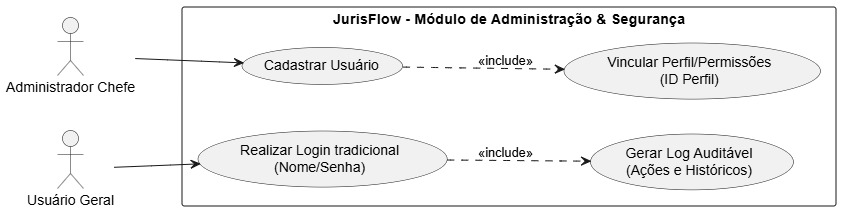
\includegraphics[width=0.9\textwidth]{04-figuras/diagrama1.jpeg}
\end{figure}

A Figura \textcolor{blue}{\ref{fig:1}}apresenta dois atores principais, com responsabilidades distintas
no sistema. O Administrador Chefe é responsável pelo cadastro de novos usuários. Nesse
processo, o caso de uso de cadastro inclui obrigatoriamente a ação de Vincular Perfil
e Permissões, identificada pelo ID do perfil, garantindo que cada usuário cadastrado
tenha as permissões correspondentes ao seu perfil de acesso. O Usuário Geral realiza o
processo de login por meio da inserção de nome e senha. Como mecanismo de segurança
e rastreabilidade, esse processo inclui automaticamente a ação de Gerar Log Auditável,
responsável por registrar as ações realizadas e o histórico de atividades do usuário no
sistema.

\begin{figure}[H]
    \centering
    \caption{Diagrama de casos de uso: Gestão de Clientes, Casos e Processos.}
    \label{fig:2}
    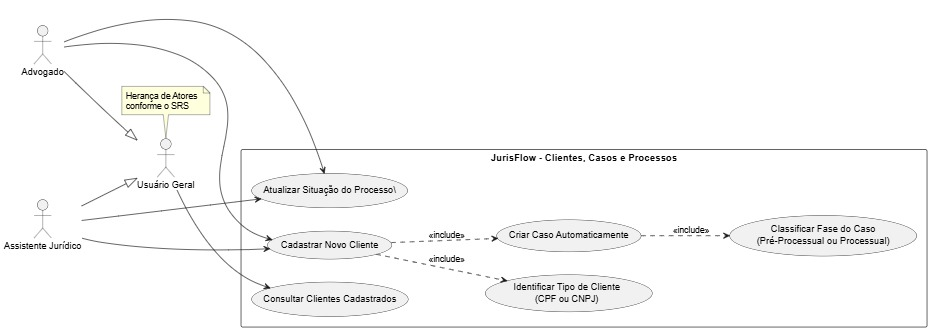
\includegraphics[width=0.9\textwidth]{04-figuras/diagrama2.jpeg}
\end{figure}
Um detalhe importante na modelagem é que tanto o Advogado quanto o Assistente
Jurídico possuem o mesmo nível de acesso e as mesmas permissões dentro deste escopo.
Ambos os profissionais podem Atualizar a Situação do Processo, Consultar Clientes
Cadastrados e iniciar o fluxo de Cadastrar Novo Cliente. Quando um dos profissionais
realiza o cadastro de um novo cliente, o sistema executa obrigatoriamente duas ações:
Identificar o Tipo de Cliente, verificando se o cadastro corresponde a CPF ou CNPJ, e
Criar Caso Automaticamente. Após a criação automática do caso, o sistema também
realiza a etapa de Classificar a Fase do Caso, definindo se o caso se encontra na fase
Pré-Processual ou Processual.

\begin{figure}[H]
    \centering
    \caption{Diagrama de casos de uso: Central de Diligências e Notificações Preventivas.}
    \label{fig:3}
    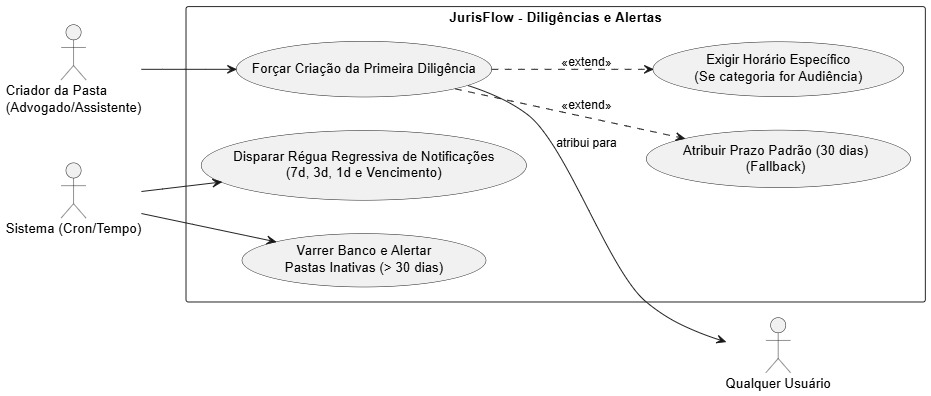
\includegraphics[width=0.9\textwidth]{04-figuras/diagrama3.jpeg}
\end{figure}

O módulo apresenta dois atores responsáveis pela interação direta com suas
funcionalidades, além de um ator de destino relacionado à execução de uma das ações.
Nesse contexto, o Criador da Pasta, representado por um Advogado ou Assistente Jurídico,
é responsável por executar a ação de Forçar Criação da Primeira Diligência, garantindo
que, após a criação da pasta, seja registrada a primeira atividade relacionada ao caso. O
fluxo também contempla duas extensões condicionais baseadas em regras de negócio. A
primeira é Exigir Horário Específico, acionada quando a categoria do caso corresponde a
uma audiência, situação na qual é necessário registrar, além da data, um horário específico
para o compromisso. A segunda é Atribuir Prazo Padrão de 30 dias, utilizada como
comportamento de fallback quando não for informado um prazo maior, garantindo que
nenhuma diligência seja criada sem uma data de vencimento definida. Além dos atores que
interagem diretamente com o módulo, existe o ator Sistema Automatizado, responsável pela
execução de rotinas em segundo plano relacionadas ao controle temporal das atividades.
Entre suas responsabilidades está Disparar a Régua Regressiva de Notificações, enviando
alertas preventivos nos períodos de 7, 3 e 1 dia antes do vencimento, bem como no próprio
dia do vencimento. O Sistema Automatizado também é responsável por Varrer o Banco e
Alertar sobre Pastas Inativas, realizando o monitoramento periódico das pastas e processos
cadastrados. Quando uma pasta permanece sem atualização por período superior a 30
dias, o sistema gera uma notificação para alertar a equipe responsável, contribuindo para
o acompanhamento contínuo dos casos e para a redução de processos sem movimentação.

\begin{figure}[H]
    \centering
    \caption{Diagrama de casos de uso:  Painel Gerencial (Métricas).}
    \label{fig:4}
    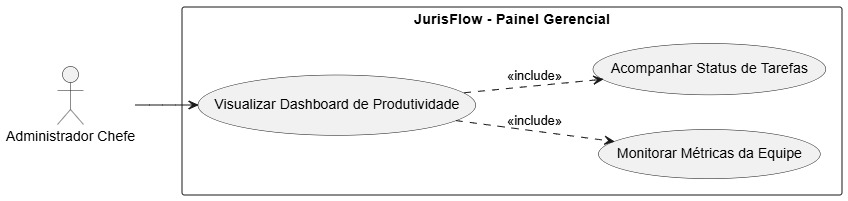
\includegraphics[width=0.9\textwidth]{04-figuras/diagrama4.jpeg}
\end{figure}

Para encerrar a apresentação dos casos de uso, o quarto diagrama representa o
módulo de Painel Gerencial (Métricas) do JurisFlow, destinado ao acompanhamento e à
supervisão das atividades do escritório. Nesse módulo, o Administrador Chefe é o ator
responsável por acessar a funcionalidade Visualizar Dashboard de Produtividade, por
meio da qual são disponibilizadas informações relacionadas ao desempenho da equipe e ao
andamento das atividades.

\section{GESTÃO E ORGANIZAÇÃO DO PROJETO}
        \include{./02-elementos-textuais/resultados}
        \include{./02-elementos-textuais/ambientes}
        \include{./02-elementos-textuais/conclusao}

\end{OnehalfSpacing}

    % -----------------------------------------------------------------------
    % ELEMENTOS PÓS-TEXTUAIS
    % -----------------------------------------------------------------------
    \postextual
    %
% Documento: Referências Bibliográficas
%

\bibliography{referencias}    % Geração automática das referências por meio do arquivo 'referencias.bib'


\end{document}